% Created by tikzDevice version 0.10.1 on 2016-04-02 12:22:54
% !TEX encoding = UTF-8 Unicode
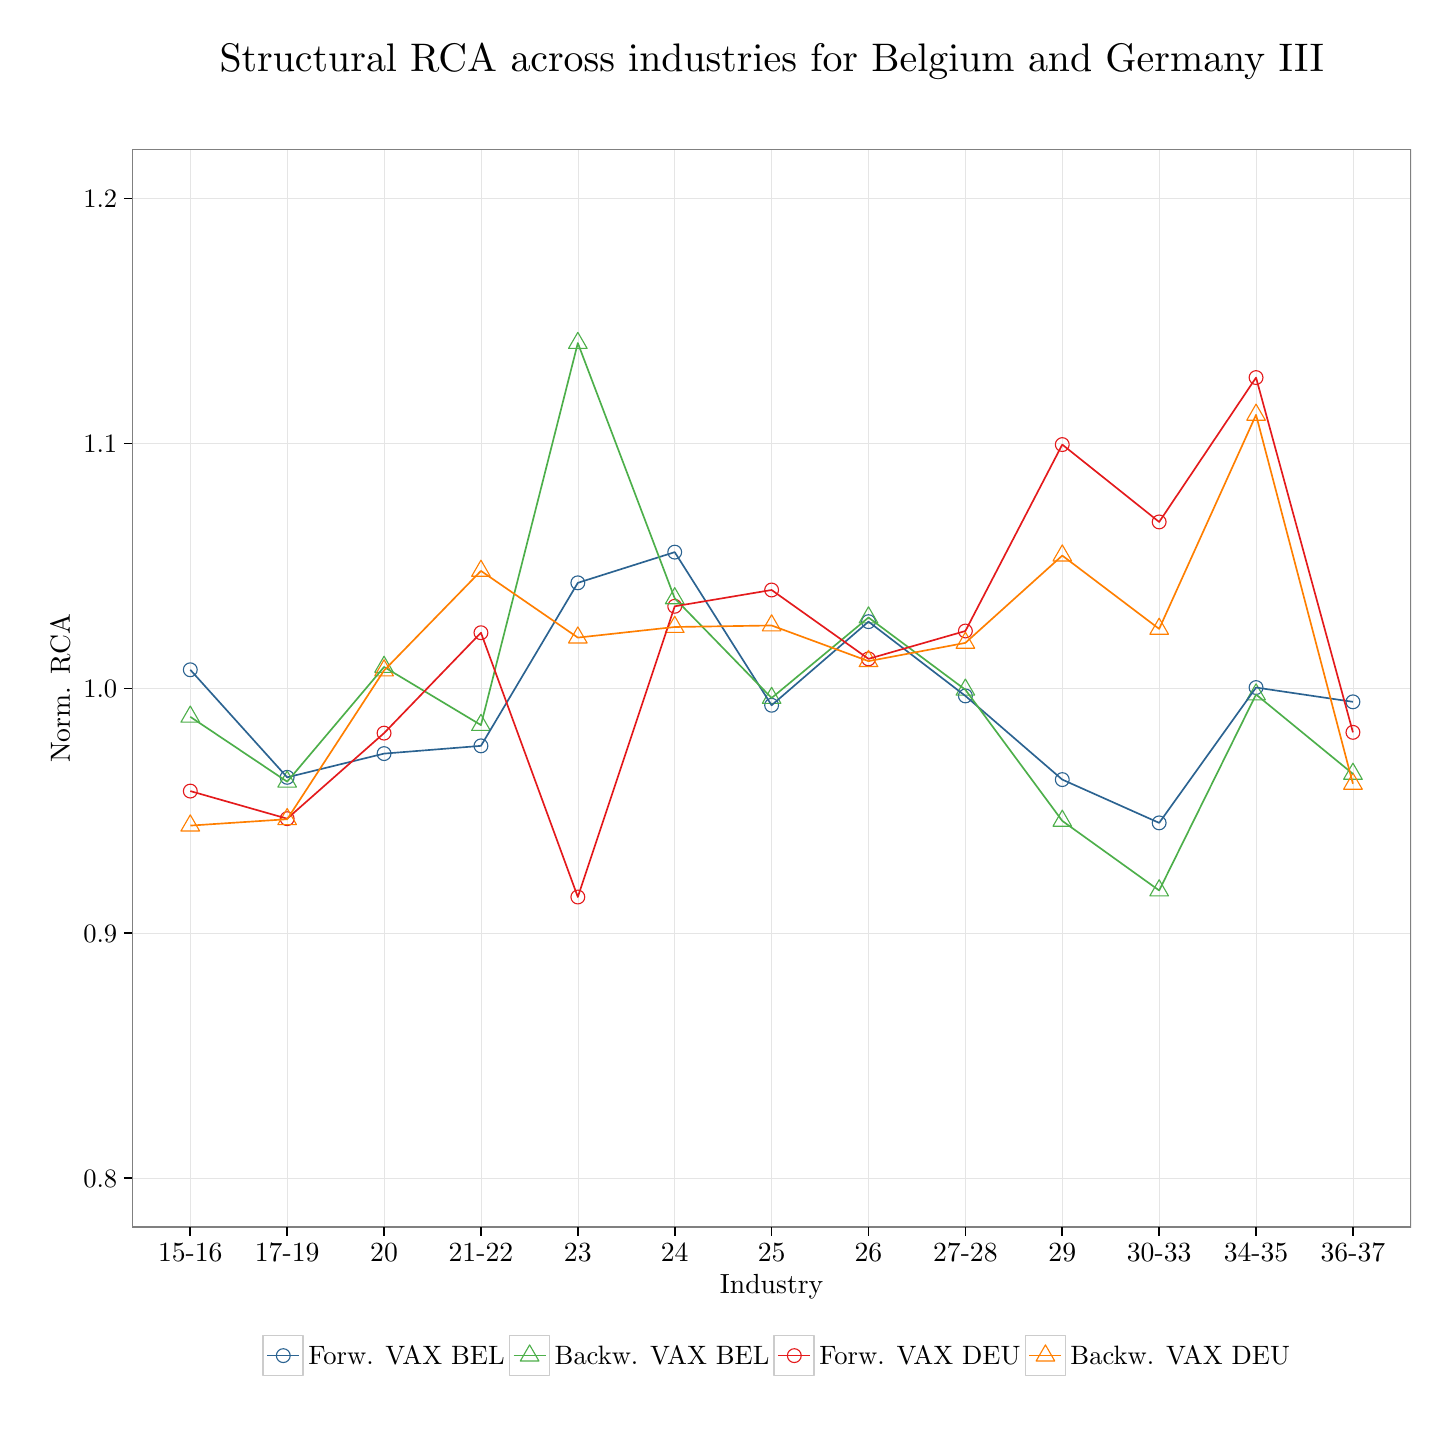
\begin{tikzpicture}[x=1pt,y=1pt]
\definecolor{fillColor}{RGB}{255,255,255}
\path[use as bounding box,fill=fillColor,fill opacity=0.00] (0,0) rectangle (505.89,505.89);
\begin{scope}
\path[clip] (  0.00,  0.00) rectangle (505.89,505.89);
\definecolor{drawColor}{RGB}{255,255,255}
\definecolor{fillColor}{RGB}{255,255,255}

\path[draw=drawColor,line width= 0.6pt,line join=round,line cap=round,fill=fillColor] (  0.00, -0.00) rectangle (505.89,505.89);
\end{scope}
\begin{scope}
\path[clip] ( 37.75, 72.44) rectangle (499.89,461.83);
\definecolor{fillColor}{RGB}{255,255,255}

\path[fill=fillColor] ( 37.75, 72.44) rectangle (499.89,461.83);
\definecolor{drawColor}{gray}{0.90}

\path[draw=drawColor,line width= 0.2pt,line join=round] ( 37.75, 90.14) --
	(499.89, 90.14);

\path[draw=drawColor,line width= 0.2pt,line join=round] ( 37.75,178.64) --
	(499.89,178.64);

\path[draw=drawColor,line width= 0.2pt,line join=round] ( 37.75,267.13) --
	(499.89,267.13);

\path[draw=drawColor,line width= 0.2pt,line join=round] ( 37.75,355.63) --
	(499.89,355.63);

\path[draw=drawColor,line width= 0.2pt,line join=round] ( 37.75,444.13) --
	(499.89,444.13);

\path[draw=drawColor,line width= 0.2pt,line join=round] ( 58.76, 72.44) --
	( 58.76,461.83);

\path[draw=drawColor,line width= 0.2pt,line join=round] ( 93.77, 72.44) --
	( 93.77,461.83);

\path[draw=drawColor,line width= 0.2pt,line join=round] (128.78, 72.44) --
	(128.78,461.83);

\path[draw=drawColor,line width= 0.2pt,line join=round] (163.79, 72.44) --
	(163.79,461.83);

\path[draw=drawColor,line width= 0.2pt,line join=round] (198.80, 72.44) --
	(198.80,461.83);

\path[draw=drawColor,line width= 0.2pt,line join=round] (233.81, 72.44) --
	(233.81,461.83);

\path[draw=drawColor,line width= 0.2pt,line join=round] (268.82, 72.44) --
	(268.82,461.83);

\path[draw=drawColor,line width= 0.2pt,line join=round] (303.83, 72.44) --
	(303.83,461.83);

\path[draw=drawColor,line width= 0.2pt,line join=round] (338.84, 72.44) --
	(338.84,461.83);

\path[draw=drawColor,line width= 0.2pt,line join=round] (373.85, 72.44) --
	(373.85,461.83);

\path[draw=drawColor,line width= 0.2pt,line join=round] (408.86, 72.44) --
	(408.86,461.83);

\path[draw=drawColor,line width= 0.2pt,line join=round] (443.87, 72.44) --
	(443.87,461.83);

\path[draw=drawColor,line width= 0.2pt,line join=round] (478.88, 72.44) --
	(478.88,461.83);
\definecolor{drawColor}{RGB}{43,99,145}

\path[draw=drawColor,line width= 0.4pt,line join=round,line cap=round] ( 58.76,273.86) circle (  2.50);

\path[draw=drawColor,line width= 0.4pt,line join=round,line cap=round] ( 93.77,235.00) circle (  2.50);

\path[draw=drawColor,line width= 0.4pt,line join=round,line cap=round] (128.78,243.57) circle (  2.50);

\path[draw=drawColor,line width= 0.4pt,line join=round,line cap=round] (163.79,246.37) circle (  2.50);

\path[draw=drawColor,line width= 0.4pt,line join=round,line cap=round] (198.80,305.28) circle (  2.50);

\path[draw=drawColor,line width= 0.4pt,line join=round,line cap=round] (233.81,316.37) circle (  2.50);

\path[draw=drawColor,line width= 0.4pt,line join=round,line cap=round] (268.82,261.04) circle (  2.50);

\path[draw=drawColor,line width= 0.4pt,line join=round,line cap=round] (303.83,291.25) circle (  2.50);

\path[draw=drawColor,line width= 0.4pt,line join=round,line cap=round] (338.84,264.42) circle (  2.50);

\path[draw=drawColor,line width= 0.4pt,line join=round,line cap=round] (373.85,234.18) circle (  2.50);

\path[draw=drawColor,line width= 0.4pt,line join=round,line cap=round] (408.86,218.54) circle (  2.50);

\path[draw=drawColor,line width= 0.4pt,line join=round,line cap=round] (443.87,267.44) circle (  2.50);

\path[draw=drawColor,line width= 0.4pt,line join=round,line cap=round] (478.88,262.28) circle (  2.50);
\definecolor{drawColor}{RGB}{228,26,28}

\path[draw=drawColor,line width= 0.4pt,line join=round,line cap=round] ( 58.76,230.03) circle (  2.50);

\path[draw=drawColor,line width= 0.4pt,line join=round,line cap=round] ( 93.77,220.06) circle (  2.50);

\path[draw=drawColor,line width= 0.4pt,line join=round,line cap=round] (128.78,250.97) circle (  2.50);

\path[draw=drawColor,line width= 0.4pt,line join=round,line cap=round] (163.79,287.25) circle (  2.50);

\path[draw=drawColor,line width= 0.4pt,line join=round,line cap=round] (198.80,191.75) circle (  2.50);

\path[draw=drawColor,line width= 0.4pt,line join=round,line cap=round] (233.81,296.80) circle (  2.50);

\path[draw=drawColor,line width= 0.4pt,line join=round,line cap=round] (268.82,302.69) circle (  2.50);

\path[draw=drawColor,line width= 0.4pt,line join=round,line cap=round] (303.83,277.81) circle (  2.50);

\path[draw=drawColor,line width= 0.4pt,line join=round,line cap=round] (338.84,287.87) circle (  2.50);

\path[draw=drawColor,line width= 0.4pt,line join=round,line cap=round] (373.85,355.24) circle (  2.50);

\path[draw=drawColor,line width= 0.4pt,line join=round,line cap=round] (408.86,327.28) circle (  2.50);

\path[draw=drawColor,line width= 0.4pt,line join=round,line cap=round] (443.87,379.45) circle (  2.50);

\path[draw=drawColor,line width= 0.4pt,line join=round,line cap=round] (478.88,251.25) circle (  2.50);
\definecolor{drawColor}{RGB}{77,175,74}

\path[draw=drawColor,line width= 0.4pt,line join=round,line cap=round] ( 58.76,260.77) --
	( 62.12,254.94) --
	( 55.39,254.94) --
	( 58.76,260.77);

\path[draw=drawColor,line width= 0.4pt,line join=round,line cap=round] ( 93.77,237.30) --
	( 97.13,231.47) --
	( 90.40,231.47) --
	( 93.77,237.30);

\path[draw=drawColor,line width= 0.4pt,line join=round,line cap=round] (128.78,278.77) --
	(132.14,272.94) --
	(125.41,272.94) --
	(128.78,278.77);

\path[draw=drawColor,line width= 0.4pt,line join=round,line cap=round] (163.79,257.76) --
	(167.15,251.94) --
	(160.43,251.94) --
	(163.79,257.76);

\path[draw=drawColor,line width= 0.4pt,line join=round,line cap=round] (198.80,395.80) --
	(202.16,389.98) --
	(195.44,389.98) --
	(198.80,395.80);

\path[draw=drawColor,line width= 0.4pt,line join=round,line cap=round] (233.81,303.55) --
	(237.17,297.73) --
	(230.45,297.73) --
	(233.81,303.55);

\path[draw=drawColor,line width= 0.4pt,line join=round,line cap=round] (268.82,267.55) --
	(272.18,261.72) --
	(265.46,261.72) --
	(268.82,267.55);

\path[draw=drawColor,line width= 0.4pt,line join=round,line cap=round] (303.83,296.63) --
	(307.19,290.80) --
	(300.47,290.80) --
	(303.83,296.63);

\path[draw=drawColor,line width= 0.4pt,line join=round,line cap=round] (338.84,270.53) --
	(342.21,264.71) --
	(335.48,264.71) --
	(338.84,270.53);

\path[draw=drawColor,line width= 0.4pt,line join=round,line cap=round] (373.85,223.15) --
	(377.22,217.32) --
	(370.49,217.32) --
	(373.85,223.15);

\path[draw=drawColor,line width= 0.4pt,line join=round,line cap=round] (408.86,198.00) --
	(412.23,192.17) --
	(405.50,192.17) --
	(408.86,198.00);

\path[draw=drawColor,line width= 0.4pt,line join=round,line cap=round] (443.87,268.82) --
	(447.24,262.99) --
	(440.51,262.99) --
	(443.87,268.82);

\path[draw=drawColor,line width= 0.4pt,line join=round,line cap=round] (478.88,240.12) --
	(482.25,234.30) --
	(475.52,234.30) --
	(478.88,240.12);
\definecolor{drawColor}{RGB}{255,127,0}

\path[draw=drawColor,line width= 0.4pt,line join=round,line cap=round] ( 58.76,221.44) --
	( 62.12,215.61) --
	( 55.39,215.61) --
	( 58.76,221.44);

\path[draw=drawColor,line width= 0.4pt,line join=round,line cap=round] ( 93.77,223.75) --
	( 97.13,217.92) --
	( 90.40,217.92) --
	( 93.77,223.75);

\path[draw=drawColor,line width= 0.4pt,line join=round,line cap=round] (128.78,277.50) --
	(132.14,271.67) --
	(125.41,271.67) --
	(128.78,277.50);

\path[draw=drawColor,line width= 0.4pt,line join=round,line cap=round] (163.79,313.47) --
	(167.15,307.65) --
	(160.43,307.65) --
	(163.79,313.47);

\path[draw=drawColor,line width= 0.4pt,line join=round,line cap=round] (198.80,289.37) --
	(202.16,283.55) --
	(195.44,283.55) --
	(198.80,289.37);

\path[draw=drawColor,line width= 0.4pt,line join=round,line cap=round] (233.81,293.21) --
	(237.17,287.38) --
	(230.45,287.38) --
	(233.81,293.21);

\path[draw=drawColor,line width= 0.4pt,line join=round,line cap=round] (268.82,293.75) --
	(272.18,287.93) --
	(265.46,287.93) --
	(268.82,293.75);

\path[draw=drawColor,line width= 0.4pt,line join=round,line cap=round] (303.83,280.87) --
	(307.19,275.04) --
	(300.47,275.04) --
	(303.83,280.87);

\path[draw=drawColor,line width= 0.4pt,line join=round,line cap=round] (338.84,287.46) --
	(342.21,281.63) --
	(335.48,281.63) --
	(338.84,287.46);

\path[draw=drawColor,line width= 0.4pt,line join=round,line cap=round] (373.85,319.01) --
	(377.22,313.18) --
	(370.49,313.18) --
	(373.85,319.01);

\path[draw=drawColor,line width= 0.4pt,line join=round,line cap=round] (408.86,292.52) --
	(412.23,286.70) --
	(405.50,286.70) --
	(408.86,292.52);

\path[draw=drawColor,line width= 0.4pt,line join=round,line cap=round] (443.87,369.86) --
	(447.24,364.04) --
	(440.51,364.04) --
	(443.87,369.86);

\path[draw=drawColor,line width= 0.4pt,line join=round,line cap=round] (478.88,236.54) --
	(482.25,230.71) --
	(475.52,230.71) --
	(478.88,236.54);
\definecolor{drawColor}{RGB}{43,99,145}

\path[draw=drawColor,line width= 0.6pt,line join=round] ( 58.76,273.86) --
	( 93.77,235.00) --
	(128.78,243.57) --
	(163.79,246.37) --
	(198.80,305.28) --
	(233.81,316.37) --
	(268.82,261.04) --
	(303.83,291.25) --
	(338.84,264.42) --
	(373.85,234.18) --
	(408.86,218.54) --
	(443.87,267.44) --
	(478.88,262.28);
\definecolor{drawColor}{RGB}{77,175,74}

\path[draw=drawColor,line width= 0.6pt,line join=round] ( 58.76,256.88) --
	( 93.77,233.42) --
	(128.78,274.88) --
	(163.79,253.88) --
	(198.80,391.92) --
	(233.81,299.67) --
	(268.82,263.67) --
	(303.83,292.74) --
	(338.84,266.65) --
	(373.85,219.26) --
	(408.86,194.12) --
	(443.87,264.93) --
	(478.88,236.24);
\definecolor{drawColor}{RGB}{228,26,28}

\path[draw=drawColor,line width= 0.6pt,line join=round] ( 58.76,230.03) --
	( 93.77,220.06) --
	(128.78,250.97) --
	(163.79,287.25) --
	(198.80,191.75) --
	(233.81,296.80) --
	(268.82,302.69) --
	(303.83,277.81) --
	(338.84,287.87) --
	(373.85,355.24) --
	(408.86,327.28) --
	(443.87,379.45) --
	(478.88,251.25);
\definecolor{drawColor}{RGB}{255,127,0}

\path[draw=drawColor,line width= 0.6pt,line join=round] ( 58.76,217.56) --
	( 93.77,219.86) --
	(128.78,273.61) --
	(163.79,309.59) --
	(198.80,285.49) --
	(233.81,289.32) --
	(268.82,289.87) --
	(303.83,276.98) --
	(338.84,283.58) --
	(373.85,315.13) --
	(408.86,288.64) --
	(443.87,365.98) --
	(478.88,232.65);
\definecolor{drawColor}{gray}{0.50}

\path[draw=drawColor,line width= 0.6pt,line join=round,line cap=round] ( 37.75, 72.44) rectangle (499.89,461.83);
\end{scope}
\begin{scope}
\path[clip] (  0.00,  0.00) rectangle (505.89,505.89);
\definecolor{drawColor}{RGB}{0,0,0}

\node[text=drawColor,anchor=base east,inner sep=0pt, outer sep=0pt, scale=  0.96] at ( 32.35, 86.83) {0.8};

\node[text=drawColor,anchor=base east,inner sep=0pt, outer sep=0pt, scale=  0.96] at ( 32.35,175.33) {0.9};

\node[text=drawColor,anchor=base east,inner sep=0pt, outer sep=0pt, scale=  0.96] at ( 32.35,263.83) {1.0};

\node[text=drawColor,anchor=base east,inner sep=0pt, outer sep=0pt, scale=  0.96] at ( 32.35,352.33) {1.1};

\node[text=drawColor,anchor=base east,inner sep=0pt, outer sep=0pt, scale=  0.96] at ( 32.35,440.83) {1.2};
\end{scope}
\begin{scope}
\path[clip] (  0.00,  0.00) rectangle (505.89,505.89);
\definecolor{drawColor}{RGB}{0,0,0}

\path[draw=drawColor,line width= 0.6pt,line join=round] ( 34.75, 90.14) --
	( 37.75, 90.14);

\path[draw=drawColor,line width= 0.6pt,line join=round] ( 34.75,178.64) --
	( 37.75,178.64);

\path[draw=drawColor,line width= 0.6pt,line join=round] ( 34.75,267.13) --
	( 37.75,267.13);

\path[draw=drawColor,line width= 0.6pt,line join=round] ( 34.75,355.63) --
	( 37.75,355.63);

\path[draw=drawColor,line width= 0.6pt,line join=round] ( 34.75,444.13) --
	( 37.75,444.13);
\end{scope}
\begin{scope}
\path[clip] (  0.00,  0.00) rectangle (505.89,505.89);
\definecolor{drawColor}{RGB}{0,0,0}

\path[draw=drawColor,line width= 0.6pt,line join=round] ( 58.76, 69.44) --
	( 58.76, 72.44);

\path[draw=drawColor,line width= 0.6pt,line join=round] ( 93.77, 69.44) --
	( 93.77, 72.44);

\path[draw=drawColor,line width= 0.6pt,line join=round] (128.78, 69.44) --
	(128.78, 72.44);

\path[draw=drawColor,line width= 0.6pt,line join=round] (163.79, 69.44) --
	(163.79, 72.44);

\path[draw=drawColor,line width= 0.6pt,line join=round] (198.80, 69.44) --
	(198.80, 72.44);

\path[draw=drawColor,line width= 0.6pt,line join=round] (233.81, 69.44) --
	(233.81, 72.44);

\path[draw=drawColor,line width= 0.6pt,line join=round] (268.82, 69.44) --
	(268.82, 72.44);

\path[draw=drawColor,line width= 0.6pt,line join=round] (303.83, 69.44) --
	(303.83, 72.44);

\path[draw=drawColor,line width= 0.6pt,line join=round] (338.84, 69.44) --
	(338.84, 72.44);

\path[draw=drawColor,line width= 0.6pt,line join=round] (373.85, 69.44) --
	(373.85, 72.44);

\path[draw=drawColor,line width= 0.6pt,line join=round] (408.86, 69.44) --
	(408.86, 72.44);

\path[draw=drawColor,line width= 0.6pt,line join=round] (443.87, 69.44) --
	(443.87, 72.44);

\path[draw=drawColor,line width= 0.6pt,line join=round] (478.88, 69.44) --
	(478.88, 72.44);
\end{scope}
\begin{scope}
\path[clip] (  0.00,  0.00) rectangle (505.89,505.89);
\definecolor{drawColor}{RGB}{0,0,0}

\node[text=drawColor,anchor=base,inner sep=0pt, outer sep=0pt, scale=  1.00] at ( 58.76, 60.15) {15-16};

\node[text=drawColor,anchor=base,inner sep=0pt, outer sep=0pt, scale=  1.00] at ( 93.77, 60.15) {17-19};

\node[text=drawColor,anchor=base,inner sep=0pt, outer sep=0pt, scale=  1.00] at (128.78, 60.15) {20};

\node[text=drawColor,anchor=base,inner sep=0pt, outer sep=0pt, scale=  1.00] at (163.79, 60.15) {21-22};

\node[text=drawColor,anchor=base,inner sep=0pt, outer sep=0pt, scale=  1.00] at (198.80, 60.15) {23};

\node[text=drawColor,anchor=base,inner sep=0pt, outer sep=0pt, scale=  1.00] at (233.81, 60.15) {24};

\node[text=drawColor,anchor=base,inner sep=0pt, outer sep=0pt, scale=  1.00] at (268.82, 60.15) {25};

\node[text=drawColor,anchor=base,inner sep=0pt, outer sep=0pt, scale=  1.00] at (303.83, 60.15) {26};

\node[text=drawColor,anchor=base,inner sep=0pt, outer sep=0pt, scale=  1.00] at (338.84, 60.15) {27-28};

\node[text=drawColor,anchor=base,inner sep=0pt, outer sep=0pt, scale=  1.00] at (373.85, 60.15) {29};

\node[text=drawColor,anchor=base,inner sep=0pt, outer sep=0pt, scale=  1.00] at (408.86, 60.15) {30-33};

\node[text=drawColor,anchor=base,inner sep=0pt, outer sep=0pt, scale=  1.00] at (443.87, 60.15) {34-35};

\node[text=drawColor,anchor=base,inner sep=0pt, outer sep=0pt, scale=  1.00] at (478.88, 60.15) {36-37};
\end{scope}
\begin{scope}
\path[clip] (  0.00,  0.00) rectangle (505.89,505.89);
\definecolor{drawColor}{RGB}{0,0,0}

\node[text=drawColor,anchor=base,inner sep=0pt, outer sep=0pt, scale=  1.00] at (268.82, 48.46) {Industry};
\end{scope}
\begin{scope}
\path[clip] (  0.00,  0.00) rectangle (505.89,505.89);
\definecolor{drawColor}{RGB}{0,0,0}

\node[text=drawColor,rotate= 90.00,anchor=base,inner sep=0pt, outer sep=0pt, scale=  1.00] at ( 15.29,267.13) {Norm. RCA};
\end{scope}
\begin{scope}
\path[clip] (  0.00,  0.00) rectangle (505.89,505.89);
\definecolor{fillColor}{RGB}{255,255,255}

\path[fill=fillColor] ( 77.26, 14.54) rectangle (460.38, 37.53);
\end{scope}
\begin{scope}
\path[clip] (  0.00,  0.00) rectangle (505.89,505.89);
\definecolor{drawColor}{gray}{0.80}
\definecolor{fillColor}{RGB}{255,255,255}

\path[draw=drawColor,line width= 0.6pt,line join=round,line cap=round,fill=fillColor] ( 85.14, 18.80) rectangle ( 99.59, 33.26);
\end{scope}
\begin{scope}
\path[clip] (  0.00,  0.00) rectangle (505.89,505.89);
\definecolor{drawColor}{RGB}{43,99,145}

\path[draw=drawColor,line width= 0.4pt,line join=round,line cap=round] ( 92.36, 26.03) circle (  2.50);
\end{scope}
\begin{scope}
\path[clip] (  0.00,  0.00) rectangle (505.89,505.89);
\definecolor{drawColor}{RGB}{43,99,145}

\path[draw=drawColor,line width= 0.6pt,line join=round] ( 86.58, 26.03) -- ( 98.15, 26.03);
\end{scope}
\begin{scope}
\path[clip] (  0.00,  0.00) rectangle (505.89,505.89);
\definecolor{drawColor}{gray}{0.80}
\definecolor{fillColor}{RGB}{255,255,255}

\path[draw=drawColor,line width= 0.6pt,line join=round,line cap=round,fill=fillColor] (174.15, 18.80) rectangle (188.60, 33.26);
\end{scope}
\begin{scope}
\path[clip] (  0.00,  0.00) rectangle (505.89,505.89);
\definecolor{drawColor}{RGB}{77,175,74}

\path[draw=drawColor,line width= 0.4pt,line join=round,line cap=round] (181.38, 29.91) --
	(184.74, 24.09) --
	(178.01, 24.09) --
	(181.38, 29.91);
\end{scope}
\begin{scope}
\path[clip] (  0.00,  0.00) rectangle (505.89,505.89);
\definecolor{drawColor}{RGB}{77,175,74}

\path[draw=drawColor,line width= 0.6pt,line join=round] (175.59, 26.03) -- (187.16, 26.03);
\end{scope}
\begin{scope}
\path[clip] (  0.00,  0.00) rectangle (505.89,505.89);
\definecolor{drawColor}{gray}{0.80}
\definecolor{fillColor}{RGB}{255,255,255}

\path[draw=drawColor,line width= 0.6pt,line join=round,line cap=round,fill=fillColor] (269.80, 18.80) rectangle (284.25, 33.26);
\end{scope}
\begin{scope}
\path[clip] (  0.00,  0.00) rectangle (505.89,505.89);
\definecolor{drawColor}{RGB}{228,26,28}

\path[draw=drawColor,line width= 0.4pt,line join=round,line cap=round] (277.02, 26.03) circle (  2.50);
\end{scope}
\begin{scope}
\path[clip] (  0.00,  0.00) rectangle (505.89,505.89);
\definecolor{drawColor}{RGB}{228,26,28}

\path[draw=drawColor,line width= 0.6pt,line join=round] (271.24, 26.03) -- (282.81, 26.03);
\end{scope}
\begin{scope}
\path[clip] (  0.00,  0.00) rectangle (505.89,505.89);
\definecolor{drawColor}{gray}{0.80}
\definecolor{fillColor}{RGB}{255,255,255}

\path[draw=drawColor,line width= 0.6pt,line join=round,line cap=round,fill=fillColor] (360.54, 18.80) rectangle (375.00, 33.26);
\end{scope}
\begin{scope}
\path[clip] (  0.00,  0.00) rectangle (505.89,505.89);
\definecolor{drawColor}{RGB}{255,127,0}

\path[draw=drawColor,line width= 0.4pt,line join=round,line cap=round] (367.77, 29.91) --
	(371.13, 24.09) --
	(364.40, 24.09) --
	(367.77, 29.91);
\end{scope}
\begin{scope}
\path[clip] (  0.00,  0.00) rectangle (505.89,505.89);
\definecolor{drawColor}{RGB}{255,127,0}

\path[draw=drawColor,line width= 0.6pt,line join=round] (361.99, 26.03) -- (373.55, 26.03);
\end{scope}
\begin{scope}
\path[clip] (  0.00,  0.00) rectangle (505.89,505.89);
\definecolor{drawColor}{RGB}{0,0,0}

\node[text=drawColor,anchor=base west,inner sep=0pt, outer sep=0pt, scale=  0.96] at (101.40, 22.72) {Forw. VAX BEL};
\end{scope}
\begin{scope}
\path[clip] (  0.00,  0.00) rectangle (505.89,505.89);
\definecolor{drawColor}{RGB}{0,0,0}

\node[text=drawColor,anchor=base west,inner sep=0pt, outer sep=0pt, scale=  0.96] at (190.41, 22.72) {Backw. VAX BEL};
\end{scope}
\begin{scope}
\path[clip] (  0.00,  0.00) rectangle (505.89,505.89);
\definecolor{drawColor}{RGB}{0,0,0}

\node[text=drawColor,anchor=base west,inner sep=0pt, outer sep=0pt, scale=  0.96] at (286.06, 22.72) {Forw. VAX DEU};
\end{scope}
\begin{scope}
\path[clip] (  0.00,  0.00) rectangle (505.89,505.89);
\definecolor{drawColor}{RGB}{0,0,0}

\node[text=drawColor,anchor=base west,inner sep=0pt, outer sep=0pt, scale=  0.96] at (376.80, 22.72) {Backw. VAX DEU};
\end{scope}
\begin{scope}
\path[clip] (  0.00,  0.00) rectangle (505.89,505.89);
\definecolor{drawColor}{RGB}{0,0,0}

\node[text=drawColor,anchor=base west,inner sep=0pt, outer sep=0pt, scale=  1.44] at ( 69.34,489.97) {Structural RCA across industries for Belgium and Germany III};
\end{scope}
\end{tikzpicture}
